%----------------------------------------------------------------------------------------
%	PACKAGES AND THEMES
%----------------------------------------------------------------------------------------

\documentclass{beamer}

\mode<presentation> {

% The Beamer class comes with a number of default slide themes
% which change the colors and layouts of slides. Below this is a list
% of all the themes, uncomment each in turn to see what they look like.

%\usetheme{default}
%\usetheme{AnnArbor}
%\usetheme{Antibes}
%\usetheme{Bergen}
%\usetheme{Berkeley}
%\usetheme{Berlin}
%\usetheme{Boadilla}
%\usetheme{CambridgeUS}
%\usetheme{Copenhagen}
%\usetheme{Darmstadt}
%\usetheme{Dresden}
\usetheme{Frankfurt}
%\usetheme{Goettingen}
%\usetheme{Hannover}
%\usetheme{Ilmenau}
%\usetheme{JuanLesPins}
%\usetheme{Luebeck}
%\usetheme{Madrid}
%\usetheme{Malmoe}
%\usetheme{Marburg}
%\usetheme{Montpellier}
%\usetheme{PaloAlto}
%\usetheme{Pittsburgh}
%\usetheme{Rochester}
%\usetheme{Singapore}
%\usetheme{Szeged}
%\usetheme{Warsaw}

% As well as themes, the Beamer class has a number of color themes
% for any slide theme. Uncomment each of these in turn to see how it
% changes the colors of your current slide theme.

%\usecolortheme{albatross}
\usecolortheme{beaver}
%\usecolortheme{beetle}
%\usecolortheme{crane}
%\usecolortheme{dolphin}
%\usecolortheme{dove}
%\usecolortheme{fly}
%\usecolortheme{lily}
%\usecolortheme{orchid}
%\usecolortheme{rose}
%\usecolortheme{seagull}
%\usecolortheme{seahorse}
%\usecolortheme{whale}
%\usecolortheme{wolverine}

%\setbeamertemplate{footline} % To remove the footer line in all slides uncomment this line
%\setbeamertemplate{footline}[page number] % To replace the footer line in all slides with a simple slide count uncomment this line

%\setbeamertemplate{navigation symbols}{} % To remove the navigation symbols from the bottom of all slides uncomment this line
}

\usepackage{graphicx, subfigure} % Allows including images
\usepackage{booktabs} % Allows the use of \toprule, \midrule and \bottomrule in tables
%\usepackage[square,sort]{natbib} % Allows citet & citep

\usepackage[utf8]{inputenc} % Accent
\usepackage[french,francais]{babel} % Français

\usepackage[scaled]{helvet}
\usepackage[sort, numbers]{natbib}

\usepackage{hyperref}

\setcitestyle{square}

\bibpunct{[}{]}{;}{a}{,}{,}

\addtobeamertemplate{navigation symbols}{}{%
    \usebeamerfont{footline}%
    \usebeamercolor[fg]{footline}%
    \hspace{1em}%
    \insertframenumber/\inserttotalframenumber
}

\addto\captionsfrench{\def\tablename{Tableau}}

% Settings des annotations ---------------------------------------------------------------
%\usepackage[disable]{todonotes} 									% notes not showed
\usepackage[draft]{todonotes}   									% notes showed

% \newcommand{\comment}[2]{#1}   									% comment not showed
\newcommand{\comment}[2]{\underline{#1}{\bfseries \color{blue}#2}}	% comment showed
% ----------------------------------------------------------------------------------------

%----------------------------------------------------------------------------------------
%	TITLE PAGE
%----------------------------------------------------------------------------------------

\title[IP exposé]{La recherche en vision artificielle \\ en France et à l'étranger}

\author{Rémi Cadène, Mickael Chen} 
\institute[UPMC]
{
Université Pierre et Marie Curie \\ % Your institution for the title page
\medskip
Exposé de l'UE Insertion Professionnelle % Your email address
}
\date{\today} % Date, can be changed to a custom date

\begin{document}

\begin{frame}
\titlepage % Print the title page as the first slide
\end{frame}

\begin{frame}
\frametitle{Sommaire} % Table of contents slide, comment this block out to remove it
\tableofcontents % Throughout your presentation, if you choose to use \section{} and \subsection{} commands, these will automatically be printed on this slide as an overview of your presentation
\end{frame}

%----------------------------------------------------------------------------------------
%	PRESENTATION SLIDES
%----------------------------------------------------------------------------------------

% sources
% http://karpathy.github.io/2012/10/22/state-of-computer-vision/
% http://www.egavves.com/a-brief-history-of-computer-vision/#sthash.zbY6gYMO.dpbs


% intro historique

% application industriels

% laboratoires et papiers

% conférences
%------------------------------------------------
%------------------------------------------------
\section{Introduction}
%------------------------------------------------
%------------------------------------------------

\begin{frame}
\frametitle{Définition de vision artificielle}

	\begin{itemize}
		\item Discipline scientifique visant à concevoir des systèmes artificiels qui acquièrent de l'information à partir d'images.
		\item Emerge dans les années 60 comme une branche de l'intelligence artificielle, s'inspirant des neurosciences computationnelles et utilisant l'apprentissage automatique.
\end{itemize}

\end{frame}

\begin{frame}
\frametitle{Des problèmes complexes posées à la machine}

\begin{figure}[H]
 \centering
 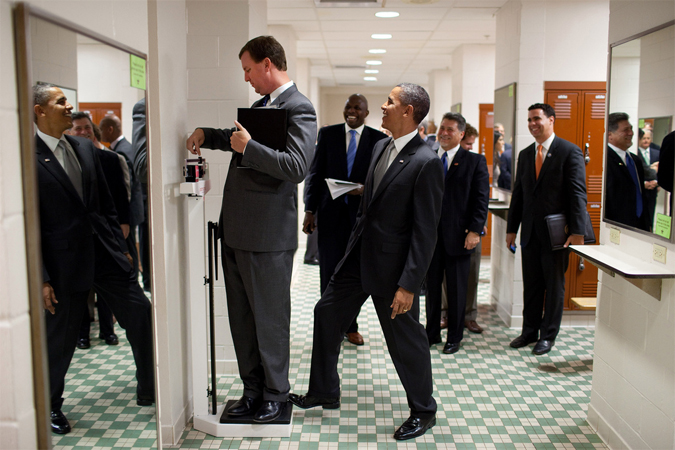
\includegraphics[width=0.7\linewidth]{img/obamafunny.jpg}
\end{figure}
\begin{itemize}
	\item Combien y a-t-il de personnes sur l'image ?
	\item Qui sont les personnes, les objets, leurs positionnements ?
	\item Est-ce que cette image est drôle ? Pourquoi ?
\end{itemize}

\end{frame}

% --- 


%------------------------------------------------
\section{Historique du domaine}
%------------------------------------------------

\begin{frame}
\frametitle{Historique des méthodes}
\begin{itemize}
\item 1958  : Perceptron de Frank Rosenblatt - entraîné à reconnaître des images de forêts avec tanks ou sans tanks (finalement juste capable de remarquer les jours ensoleillés)
\item années 90 : Convolutional Networks - reconnaissance des chiffres sur les chèques bancaires, mais incapable de fonctionner sur des problèmes plus complexes
\item années 2000 : Bag Of visual Word, SIFT, SVM - classification et détection d'objets, moteur de recherche d'images, reconnaissance faciale
\item 2012 : AlexNet - émergence du Deep Learning grâce aux implémentations GPUs - état de l'art sur des bases de données moyennes et grandes
\end{itemize}

\end{frame}

\begin{frame}
\frametitle{Historique des conférences}

\begin{itemize}
\item 1968 Journal: Pattern Recognition (Pergamon, Elsevier)
\item 1969 Textbook : Picture Processing by Computer (A. Rosenfeld)
\item 1970 International Conference on Pattern Recognition (ICPR)
\item 1977 Computer Vision and Pattern Recognition (CVPR)
\item 1978 International Association for Pattern Recognition (IAPR)
\item 1979 IEEE Transactions on Pattern Analysis and Machine Intelligence (PAMI)
\item 1980 International Conference on Machine Learning (ICML)
\item 1987 International Conference on Computer Vision (ICCV)
\item 1987 Neural Information Processing Systems (NIPS)
\item 1990 European Conference on Computer Vision (ECCV)
\end{itemize}

\end{frame}

%http://pages.isir.upmc.fr/~bredeche/Teaching/IAR/

%------------------------------------------------
\section{Travaux en recherche et applications dans l'industrie}
%------------------------------------------------

\begin{frame}
\frametitle{Quelques applications industrielles}

\begin{tabular}{r l}
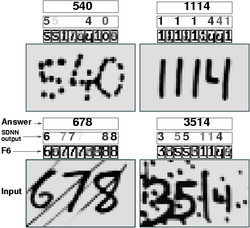
\includegraphics[width=0.4\linewidth]{img/sdnn-2.png} & 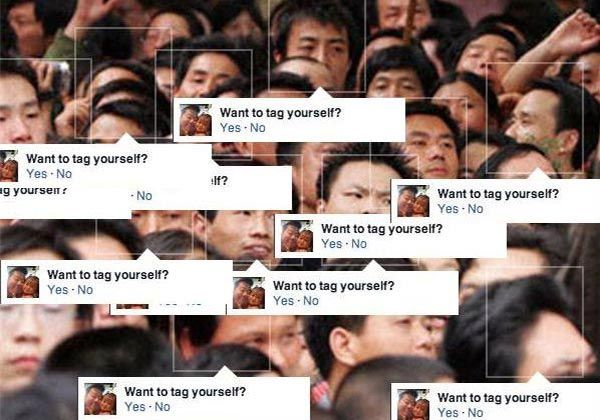
\includegraphics[width=0.5\linewidth]{img/facereco.jpg} \\
 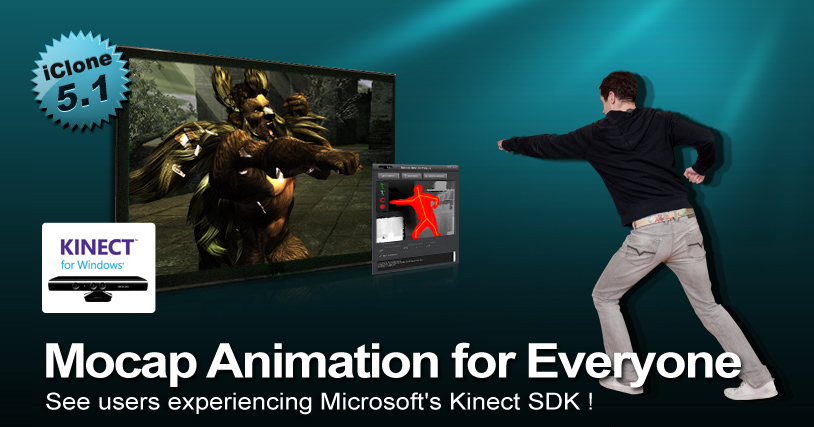
\includegraphics[width=0.4\linewidth]{img/kinect.jpg} &  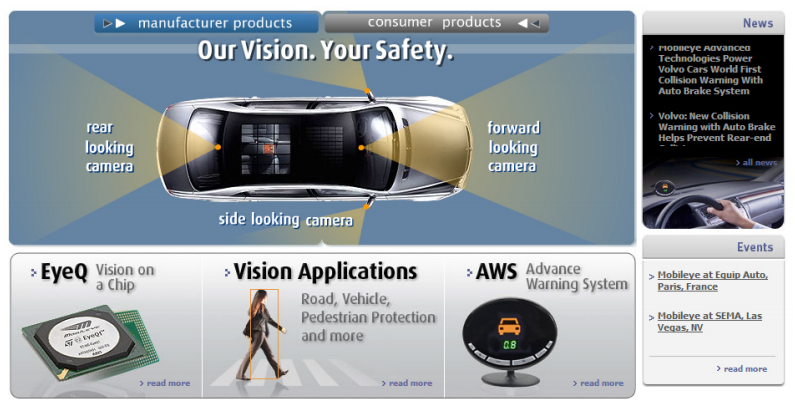
\includegraphics[width=0.6\linewidth]{img/smart_cars.png}
\end{tabular}

\end{frame}

\begin{frame}
\frametitle{Projets en cours d'industrialisation}
\begin{tabular}{r l}
 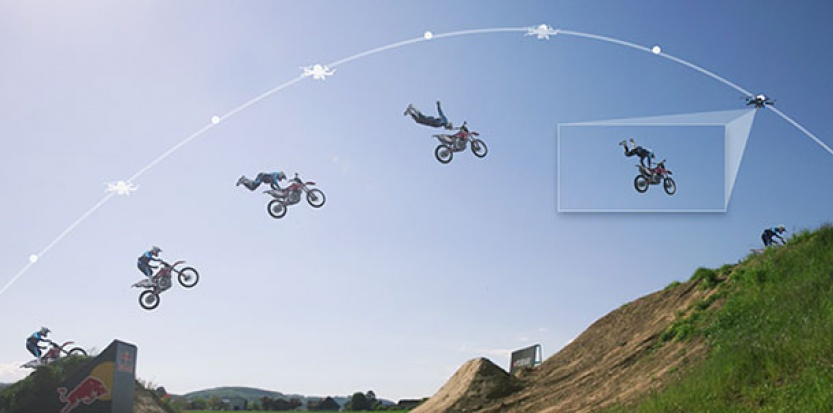
\includegraphics[width=0.5\linewidth]{img/dronetracking.jpg} &
 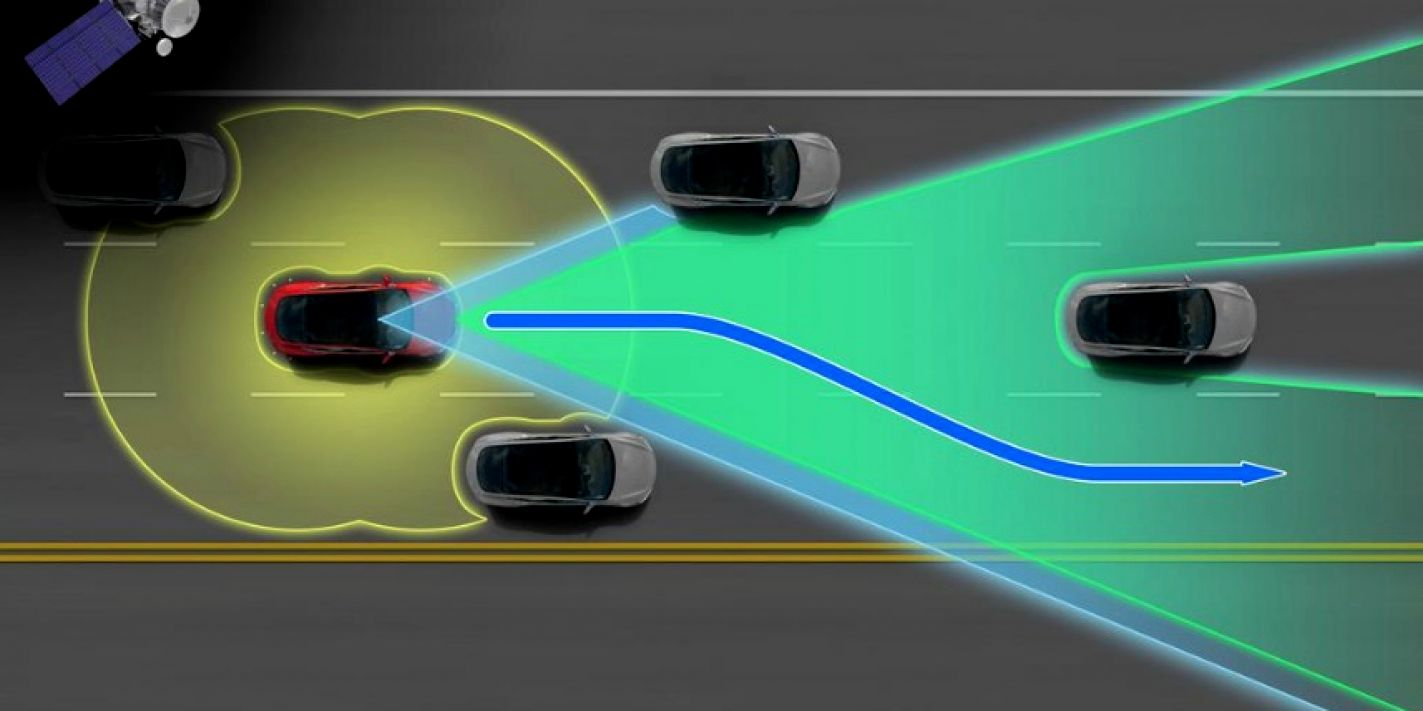
\includegraphics[width=0.5\linewidth]{img/tesla.jpg} \\
 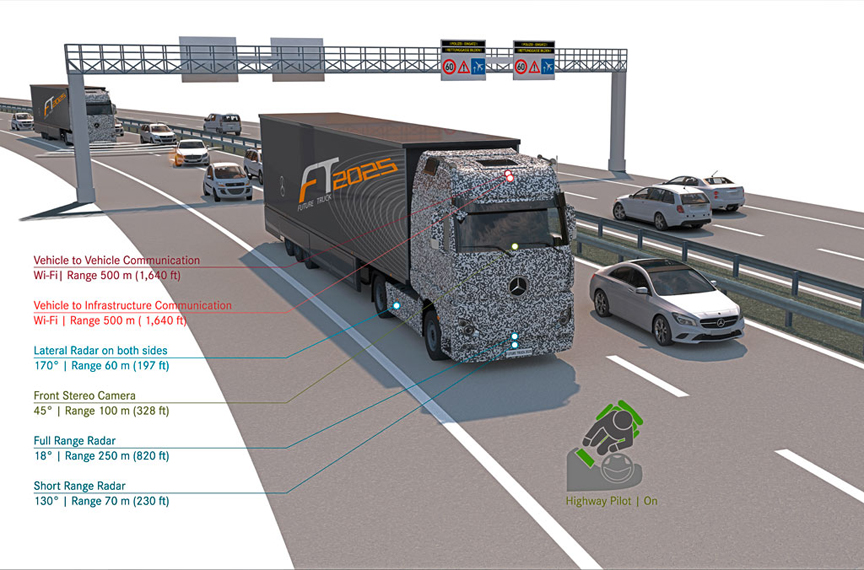
\includegraphics[width=0.5\linewidth]{img/selfdrivingtruck.jpg} &
 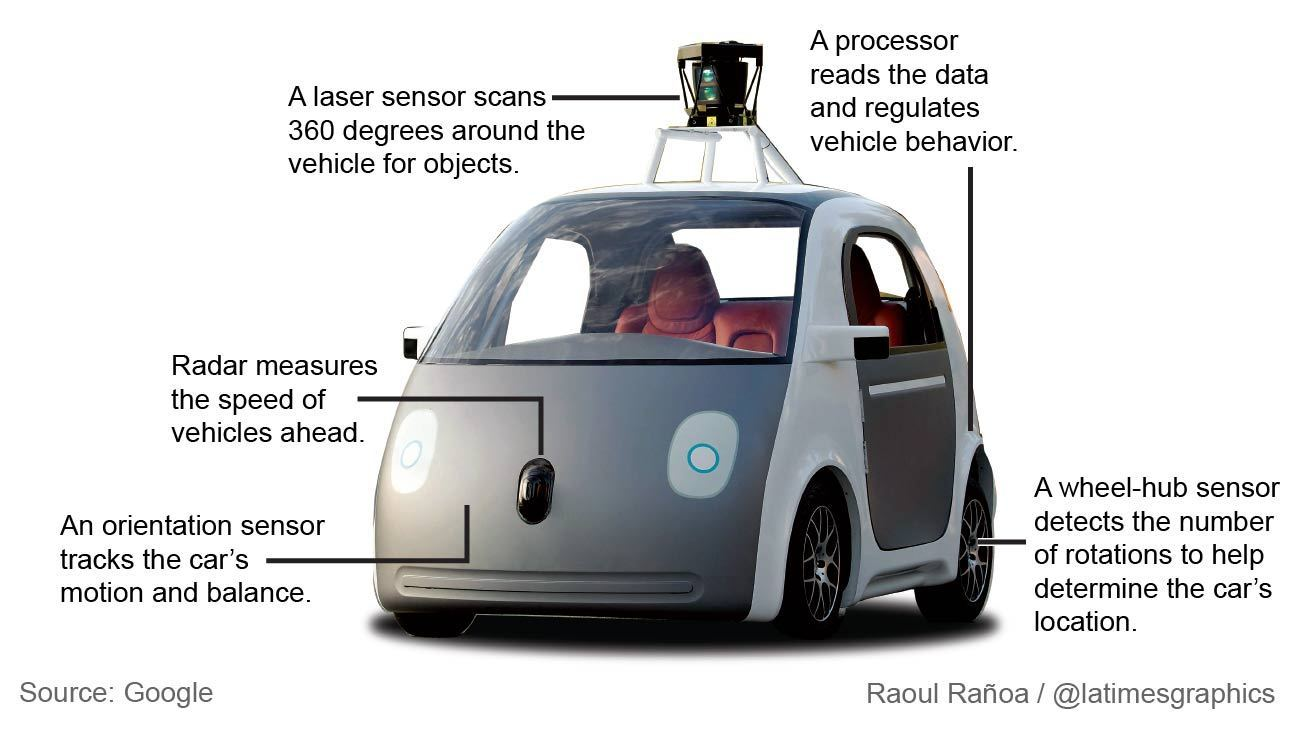
\includegraphics[width=0.5\linewidth]{img/googlecar.jpg} 
\end{tabular}
\end{frame}

% \url{http://cs.stanford.edu/people/karpathy/deepimagesent/}

\begin{frame}
\frametitle{Travaux de recherche récents}

\begin{figure}[H]
 \centering
 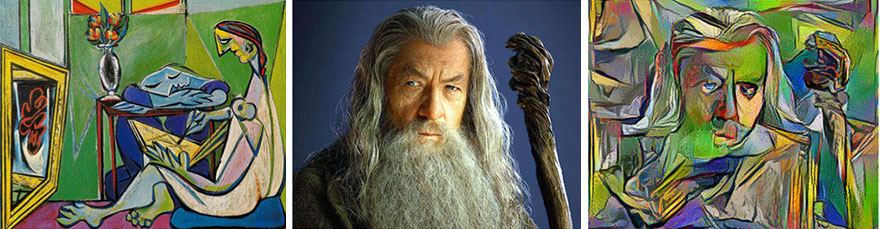
\includegraphics[width=0.8\linewidth]{img/artisticnet2.jpg}
\end{figure}

\begin{tabular}{r c}
 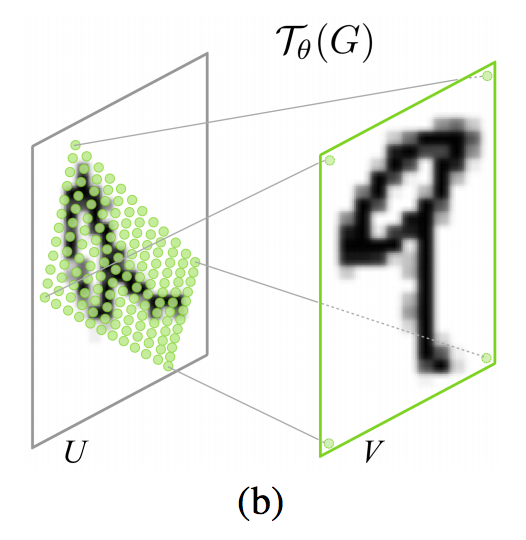
\includegraphics[width=0.4\linewidth]{img/spatialtransformernet.png} &
 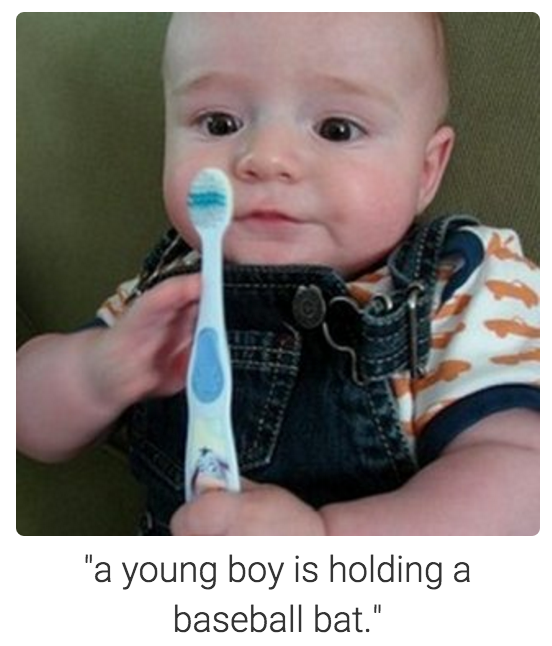
\includegraphics[width=0.4\linewidth]{img/deepimagesent.png}
\end{tabular}
\end{frame}


% --- 
\iffalse
\begin{frame}
\frametitle{ECCV}

European Conference on Computer Vision

Fréquence : biannuelle

Site web : \url{http://eccv2014.org/}

\end{frame}

\begin{frame}
\frametitle{ICCV}

International Conference on Computer Vision

Site web : \url{http://pamitc.org/iccv15/}

\end{frame}

\begin{frame}
\frametitle{CVPR}

\end{frame}

\begin{frame}
\frametitle{ICPR}

\end{frame}

\begin{frame}
\frametitle{ICML}


\end{frame}

\begin{frame}
Computer vision
ICCV
CVPR
ICPR
ECCV

Machine Learning
ICML
\end{frame}
\fi

%------------------------------------------------
\section{Laboratoires de recherche en France et à l'étranger}
%------------------------------------------------

\iffalse
\begin{frame}
\frametitle{LIP6 - MLIA}

Équipe de recherche en Computer Vision: 
\begin{itemize}
\item Matthieu Cord (Professeur)
\item Nicolas Thome (HDR)
\item 4 doctorants 
\end{itemize}

\begin{figure}[H]
 \centering
 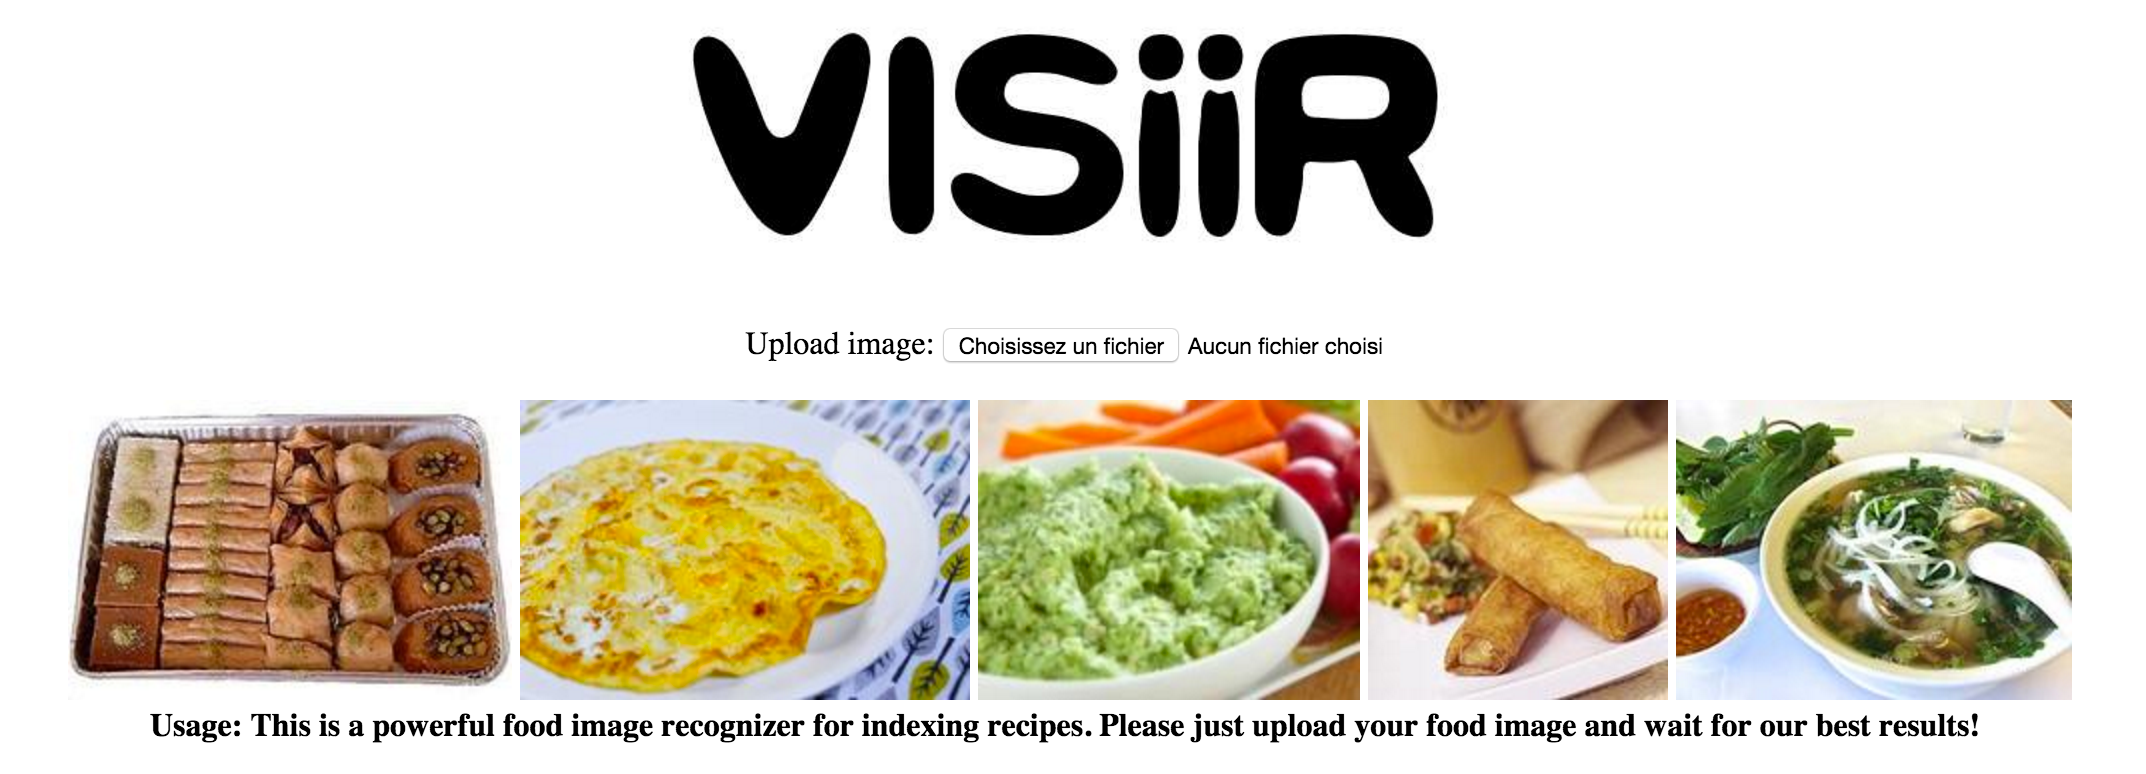
\includegraphics[width=0.8\linewidth]{img/visiir.png}
\end{figure}

\end{frame}
\fi

% ---

\begin{frame}
\frametitle{Laboratoires influents français}

\begin{itemize}
\item LIP6 (Paris) : Laboratoire d'Informatique de Paris 6 (équipe MLIA)
\item LIRIS (Lyon) : Laboratoire d'Informatique en Image et Systèmes d'information \url{https://liris.cnrs.fr}
\item LIG (Grenoble) : Laboratoire d'Informatique de Grenoble \url{http://www.liglab.fr/}
\item IRIT (Toulouse) : Institut de Recherche en Informatique de Toulouse \url{http://www.irit.fr/}
\end{itemize}

\end{frame}


\begin{frame}
\frametitle{Laboratoires influents dans le monde}
\begin{itemize}
\item SAIL - Stanford Artificial Intelligence Lab \\
ImageNet [L. Fei Fei]
\item NYU - New York University Vision Learning Graphics \\
ConvNet, MNIST [Y. Lecun]
\item UoTML - University of Toronto Machine Learning \\
Neural Network [G. Hinton]
\item LISA - Université de Montréal \\
Deep Learning [Y. Bengio]
\item ICVL - Imperial Computer Vision \& Learning Lab
\item VGG - Oxford Visual Geometry Group 

\end{itemize}
\end{frame}


\begin{frame}
\frametitle{La recherche privé}

\begin{itemize}
\item AT\&T Bell Labs: Historique
\item Google Deep Mind (Londres): Renforcement, réseaux récurrent, image
\item Facebook AI (Paris): Reconnaissance de visage et contexte
\item Google: Moteur de recherche d'image, Vidéo, Captionning
\item Baidu Research (Sunnyvale, California), Microsoft, Adobe, Twitter...
\item US Army Research Laboratory, Thalès...
\item NVIDIA: Implémentation GPU
\end{itemize}

\end{frame}

% ---
\iffalse
\begin{frame}
\frametitle{Google Deep Mind}

Fondé en 2010, acquis par Google en 2014.

Ville : Londres

Thèmes : Machine Learning (RNN, CNN) and Systems Neuroscience

Publications : Nature, ICML, eLife, ICLR, ICML, IJCAI, AISTATS, AAAI, ACL, NIPS, Neuron

Site web : \url{http://deepmind.com/}
\end{frame}

% -- 

\begin{frame}
\frametitle{Facebook AI Research}

Villes : Paris, New York City, Menlo Park (California)

Site web : \url{https://research.facebook.com/ai}

\end{frame}
\fi

\section{Conclusion}

\begin{frame}
\frametitle{Conclusion}
	\begin{itemize}
		\item Un domaine en plein essor, interconnecté avec celui de l'apprentissage artificiel
        \item Une recherche publique active en Europe et en Amérique du Nord, très liés aux milieux industriels
        \item Quelles conséquences sur la société ? (Voitures automatiques, Tracking de visages, Drone de surveillance...)
	\end{itemize}

\end{frame}


%------------------------------------------------

\begin{frame}
\frametitle{Bibliographie}

\nocite{Karpathy}
% http://karpathy.github.io/2012/10/22/state-of-computer-vision/

\nocite{karpathy2014deep}
% http://cs.stanford.edu/people/karpathy/deepimagesent/

\nocite{Gavves}
% http://www.egavves.com/a-brief-history-of-computer-vision/#sthash.zbY6gYMO.dpbs

\nocite{ICML}
% https://en.wikipedia.org/wiki/International_Conference_on_Machine_Learning

\nocite{Hays}
% https://cs.brown.edu/courses/cs143/lectures/01.pdf

\nocite{Huang}
% https://cds.cern.ch/record/400313/files/p21.pdf

\nocite{Hoiem}
% http://dhoiem.cs.illinois.edu/courses/vision_spring10/lectures/Lecture1%20-%20Introduction.pdf

\nocite{Tesla}
% http://www.teslamotors.com/blog

\nocite{jaderberg2015}

%\bibliographystyle{plain}
%\bibliography{bibtex}
%\printbibliography

\bibliographystyle{apalike}
\tiny\bibliography{bib.bib}

\end{frame}



\end{document}